\documentclass{article} % For LaTeX2e
\usepackage{cos424,times}
\usepackage{url}
\usepackage{graphicx}
\usepackage{hyperref}
\usepackage{multirow}
\usepackage{amsmath}
\usepackage{listings}
\usepackage{csquotes}
\usepackage{subcaption}
\usepackage{multirow}

\lstset{
    basicstyle=\small\ttfamily,
    columns=flexible,
    breaklines=true
}

\title{Predicting transactions in Bitcoin blockchain data}

\author{
Gregory Gundersen\\
Princeton University\\
\texttt{ggundersen@princeton.edu}
\And
Prakhar Kumar \\
Princeton University \\
\texttt{prakhark@princeton.edu} \\
}

\newcommand{\fix}{\marginpar{FIX}}
\newcommand{\new}{\marginpar{NEW}}

\begin{document}

\maketitle

\begin{abstract}
We predict future Bitcoin transactions for pairs of addresses based on historical transaction data. The training dataset consists of transaction counts between sender-receiver address pairs that interacted within a one-year period. The test data consists of address pairs which did not interact within that one year period but may have in the future. We approach the problem in two ways: supervised learning on a subsample of a full dataset of graph features and matrix completion of an extremely sparse adjacency matrix. We find that two supervised classifiers, support vector machine with a linear kernel and logistic regression, and two matrix completion methods, singular value decomposition and nonnegative matrix factorization, generalize significantly better than random guessing.
\end{abstract}

\section{Introduction}

\subsection{Background}

Bitcoin is an online virtual currency introduced in 2008 by Satoshi Nakamoto \cite{nakamoto2008bitcoin}. All transactions are cryptographically signed and recorded on a public ledger called the blockchain. The blockchain allows the global, peer-to-peer network of Bitcoin users to validate all transactions and thereby eschew a centralized bank. See \cite{nielsen2013bitcoin} for a detailed explanation of how Bitcoin works. The upshot is that with Bitcoin, everyone is the bank and the blockchain is an account of the entire history of all anonymized transactions.

In this paper, we predict transactions between pairs of addresses in a portion of the Bitcoin blockchain. The training dataset consists of transaction counts between sender-receiver address pairs that did interact, i.e. there are no zero counts, within a one year period. Therefore the entire training dataset consists of positive examples. The testing dataset consists of some pairs of addresses which did not interact and some which did in a subsequent year. In particular, we investigate two matrix completion methods, singular value decomposition (SVD) and nonnegative matrix factorization (NMF). Their performances were evaluated on accuracy, precision, recall, and area under the curve (AUC). We found that NMF generalizes better on the test data in comparison to SVD. We also explored latent Dirichlet allocation (LDA) but the method was slow with worse performance.

We also explored an alternative approach to the prediction problem by using traditional, supervised classifiers, SVM and logistic regression. For this purpose, we extracted features from the training dataset using graph properties of indegree and outdegree for each node corresponding to each address. Using nonzero counts of transactions as positive labels, we trained the models for both these classifiers by constructing a subsample of the full dataset consisting of address pairs which did not interact in the training dataset along with the ones that did. We observed that these two methods performed equally well as compared to the matrix completion methods described above.

\subsection{Related work}

Matrix completion methods are frequently used for recommender systems \cite{koren2009matrix}. This is because recommender systems typically rely on incomplete and/or sparse data to provide suitable recommendations to the users for services like Amazon, Facebook, and Netflix. The sparsity is common because in most scenarios a user cannot rate or even be aware of most items. The central challenge, then, is to develop methods to fill in missing recommendations based on the user and others' recommendations. The key assumption is that user preferences are generally guided by a small number of underlying factors and so decomposing the data into a low-rank representation creates a more general model. The Netflix Prize is a popular example of recommender systems employing large scale SVD and other matrix completion methods to estimate the probable preferences of users for movies \cite{bennett2007netflix}.

This approach can be used for predicting Bitcoin transactions because we assume the number of factors which determine whether or not two users will interact is much smaller than the number of addresses in the dataset. The significant sparsity of our dataset makes it ideal to implement matrix factorization methods for identifying low-rank decompositions of the original data.

\section{Methods}

\subsection{Data}

\paragraph{Description.} The training dataset consists of transactions between 3,348,026 sender-receiver pairs and the number of times the sender paid the receiver. The transactions were made between March 2012 and March 2013. The testing dataset consists of sender-receiver pairs which did not interact in the training set time period but may have by the following year, May 2014. The full dataset contains 444,075 unique addresses, and therefore over 19.7 billion possible unordered pairs of addresses. An adjacency matrix is extremely sparse, with only $1.7 \times 10^{-5}$ nonzero values.

\paragraph{Exploration.} To better understand the data, we constructed a smaller dataset with three columns: address, outdegree, and indegree. We found a positive correlation between indegree and outdegree (Figure \ref{fig:degree_address}). Surprisingly, while some nodes have high outdegree without a high indegree, no nodes have a high indegree but a low outdegree. We expected the opposite: online merchants would receive many payments but not send money often.

In addition, we also found a strong relationship between the address and the outdegree (Figure \ref{fig:in_out_degree}) and indegree (not shown). Lower address numbers have higher indegrees and outdegrees. This suggests that the addresses themselves will be useful as features.

\begin{figure}
\centering
\begin{subfigure}{.5\textwidth}
    \centering
    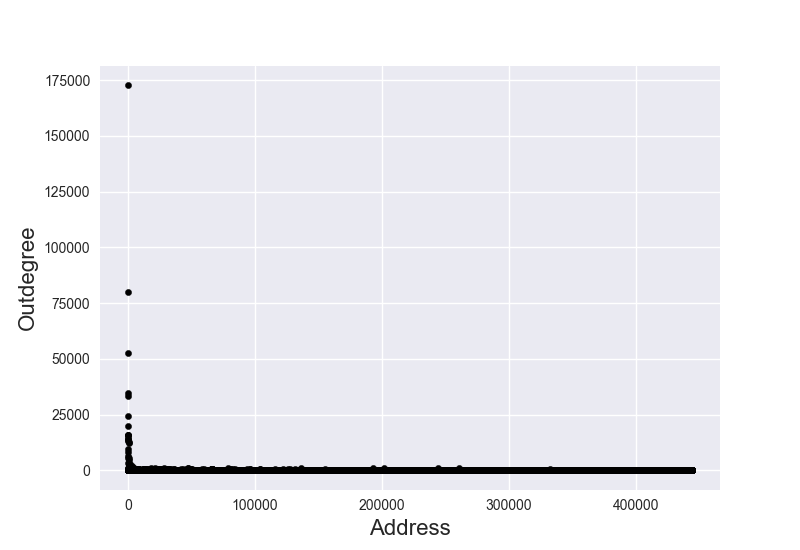
\includegraphics[width=1\linewidth]{figures/degree_address}
    \caption{\small Relationship between outdegree and address. We would have expected there to be no relationship.}
    \label{fig:degree_address}
\end{subfigure}%
\begin{subfigure}{.5\textwidth}
    \centering
    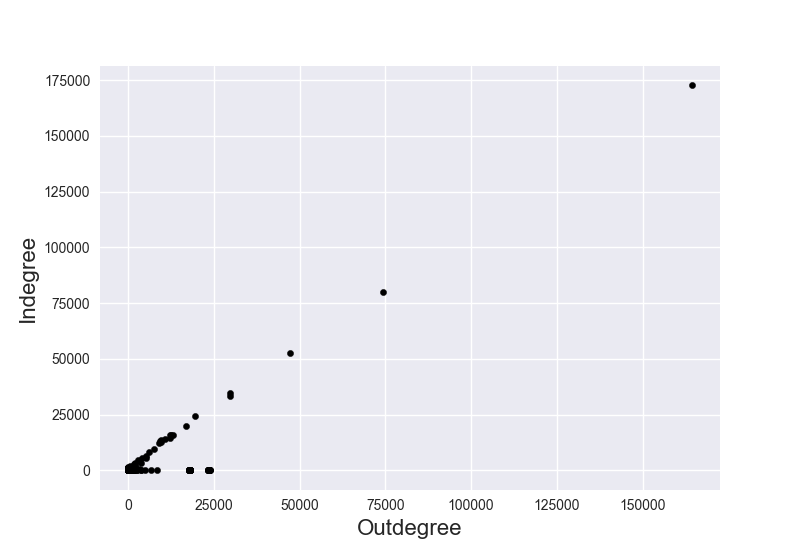
\includegraphics[width=1\linewidth]{figures/in_out_degree}
    \caption{\small Relationship between indegree and outdegree.}
    \label{fig:in_out_degree}
\end{subfigure}
\caption{\small Exploring the graph-related features of the dataset.}
\label{fig:test}
\end{figure}

\subsection{Features}\label{features}

We approached prediction through two views of the data: matrix completion of an adjacency matrix and supervised learning on a dataset with graph properties as features.

For matrix completion, the dataset is a $444,075 \times 444,075$ adjacency matrix, far too large to store in memory. We used the Python library \texttt{scipy} for several representations of sparse matrices which work with \texttt{scikit-learn}'s SVD, NMF, and LDA implementations \cite{jones2014scipy} \cite{scikit-learn}.

For supervised learning, we generated a new dataset with six features of the implicit graph in the transaction dataset: (1) sender address, (2) receiver address, (3), sender outdegree, (4) sender indegree, (5) receiver outdegree, and (6) receiver indegree. The number of transactions was dropped from the training dataset because it is not available in the test dataset. We tested two supervised classifiers on this dataset, SVM and logistic regression.

\subsection{Classifiers}\label{classifiers}

\paragraph{Spotlight: Nonnegative matrix factorization.}\label{Spotlight}

NMF is a method for approximating a matrix as the outer product of two other, typically smaller, matrices. Formally, a matrix $X$ is factorized into matrices $V$ and $U$ such that:

\begin{equation}\label{eq:1}
X \approx V \times U
\end{equation}

Where $X$ is an $n \times m$ matrix, $V$ is an $n \times k$ matrix, and $U$ is a $k \times m$ matrix. The value $k$ is a hyperparameter of the model which indicate the number of latent variables that approximate $X$ (Figure \ref{fig:matrix_completion}).

\begin{figure}[!htbp]
    \centering
    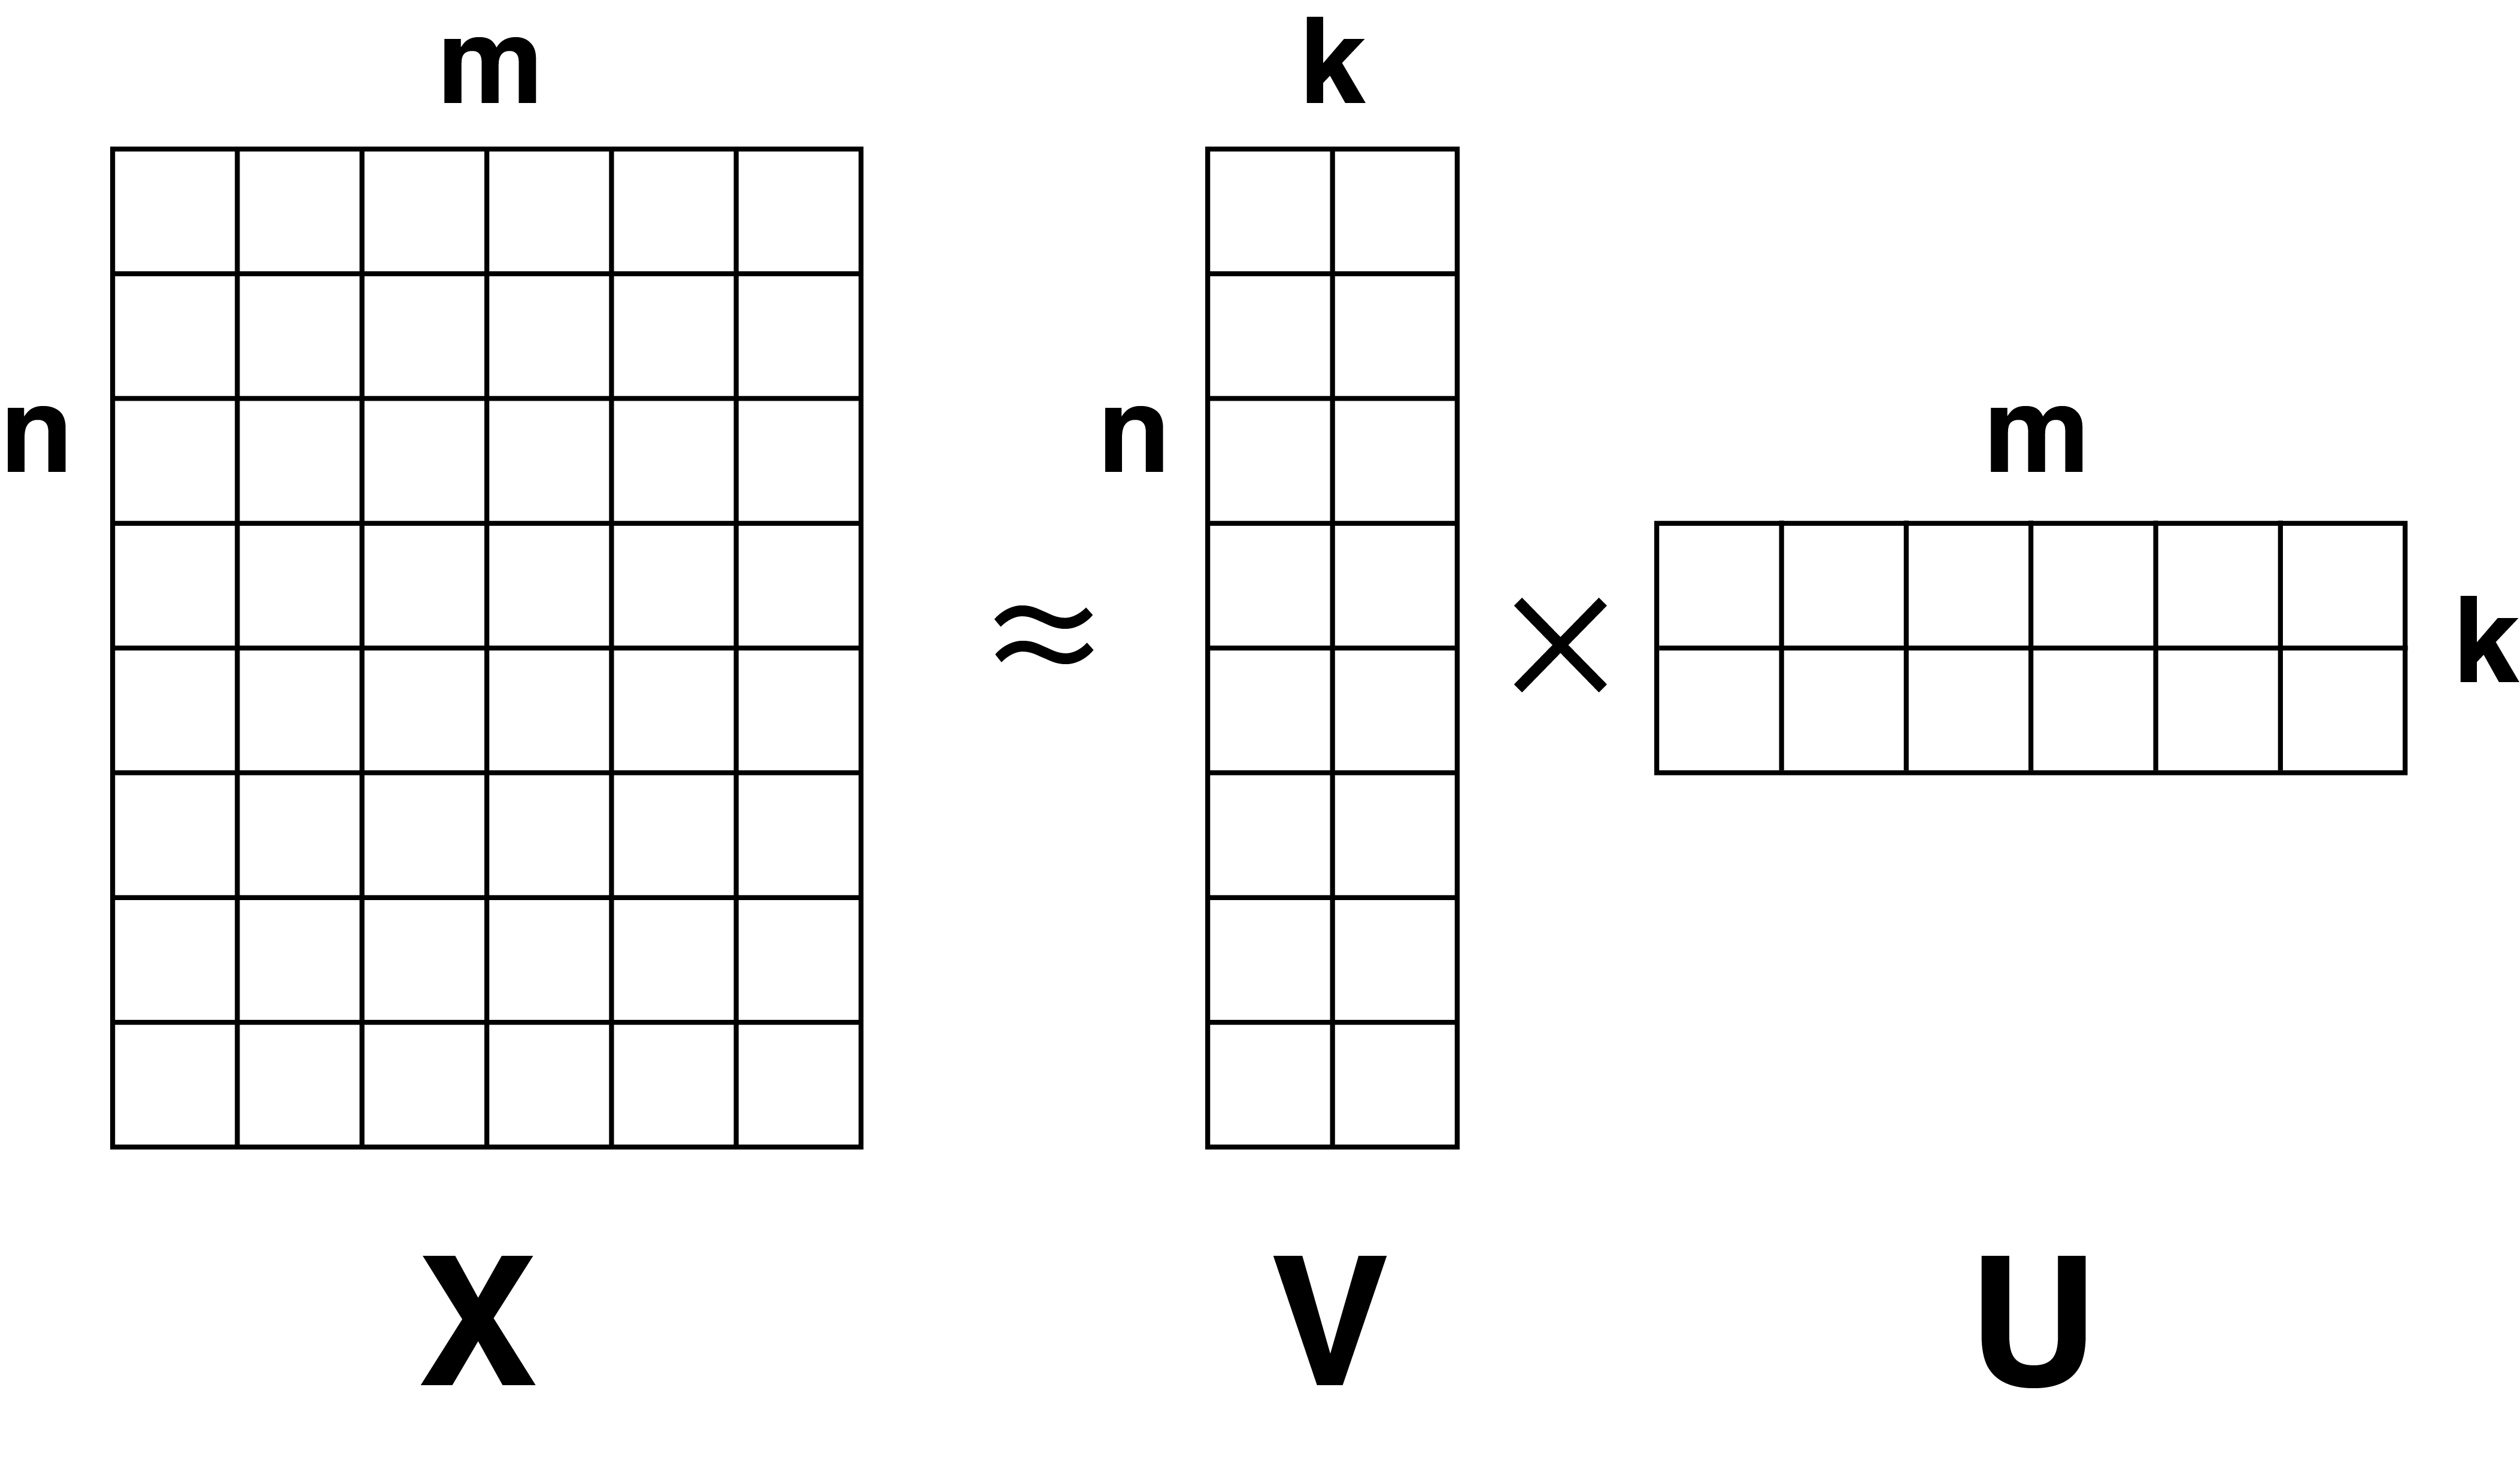
\includegraphics[scale=0.2]{figures/matrix_completion}
    \caption{\small Matrix $X$ is factorized into matrices $V$ and $U$.}
    \label{fig:matrix_completion}
\end{figure}

The key assumption is that the approximated matrix has low-rank. In other words, not every cell in the matrix is a free variable. Instead, each cell value is the dot product of two $k$-dimensional vectors which are shared with other cells. The value of the low-rank assumption is that it reduces the number of free parameters of a model. In the most extreme case, $k=1$, a model that would typically have $n \times m$ parameters can be approximated by just $n + m$ parameters. In general, the number of parameters is $k \times (n + m)$.

Prediction for matrix completion methods such as NMF are as follows. First, we approximate the observed data $X$ using matrix factorization (Equation \ref{eq:1}). We then complete the matrix by multiplying the two matrix factors together:

\begin{equation}
\hat{X} = V \times U
\end{equation}

In principle, $\hat{X}$ is a matrix that captures the latent structure in $X$. We can then base predictions on the values in the completed matrix. For example, the prediction for whether or not the $i$th address made a transaction with the $j$th address would be found in cell $\hat{X}[i, j]$.

There are many algorithms for solving matrix factorization for NMF \cite{lee2001algorithms}. One straightforward way is to use gradient descent to minimize the difference between the observed data and the factorized estimates. Formally, given observation $X_{ij}$, we want to find low-dimensional vectors $v$ and $u$ such that $X_{ij} = v_i \cdot  u_j$ by minimizing the following objective function:

$$
f(u, v) = \sum_{i,j \text{ observed}} (X_{ij} - v_i \cdot u_j)^2
$$

Ultimately, the learned matrices $V$ and $U$ are uninterpretable. But like many machine learning methods, we assume that if we can approximate the data well with fewer numbers, we might capture generalities in the data. Other dimensionality reduction methods such as SVD and PCA rely on this thinking as well.

\paragraph{Classifiers.} We used five classifiers from the \texttt{scikit-learn} Python library \cite{scikit-learn}, two which perform supervised learning on graph features and two which use matrix completion. Unless stated otherwise, we used the default parameters for each classifier as implemented by \texttt{scikit-learn}.

\emph{Supervised learning classifiers.} For both supervised learning models, the full dataset was too large. Instead, we trained each model on random subsamples of the full dataset. In each experiment, the size of the subsample was 1,000,000. We varied the percentage of positive examples in each subsample ($pp$) and report the results in Table \ref{tab:standardresults}.

\begin{itemize}

    \item \textbf{Linear Support Vector Machine} (LSVM): A linear SVM classifier finds a hyperplane which maximizes the distance of the hyperplane from the data being classified. Since \texttt{scikit-learn}'s default \texttt{SVC} class was extremely slow, we trained a \texttt{SGDClassifier} model, which is a linear classifier trained with stochastic gradient descent. We used the hinge loss function, which makes the model equivalent to linear SVM. We trained it online for 100 batches with a batch size of 100000 and 0.1\% positive examples.

    \item \textbf{Logistic Regression} (LR): Logistic regression is regression with binary labels. We used \texttt{scikit-learn}'s \text{\detokenize{predict_proba}} function to get probabilities for the ROC curve and used a threshold for prediction of 0.5.

\end{itemize}

\emph{Matrix completion methods.}

\begin{itemize}

    \item \textbf{Singular Value Decomposition.} (SVD): SVD is a matrix factorization and dimensionality reduction technique. It decomposes the original data into a product of 3 matrices: $U$, $\Sigma$ and $V$ where $\Sigma$ is a diagonal matrix while $U$ and $V$ are left-singular and right-singular matrices respectively. In order to decompose the large sparse data matrix as a product of two low-rank matrices using SVD, we analyzed the singular values by plotting these singular values for different components. We decided to select the top 20 components by observing a “knee” in the plot (Figure \ref{fig:svd}). Thus, the assumption was that the basic factors determining whether a transaction would take place can be explained by these 20 components.

    \item \textbf{Nonnegative Matrix Factorization} (NMF): NMF decomposes multivariate data into the product of two non-negative matrices. By restricting the rank of the matrices, we can create a dense, low-rank approximation of the data. See Section \ref{Spotlight} for details.

    \item \textbf{Latent Dirichlet Allocation} (LDA): LDA builds a low-rank approximation of the data by using small number of ``topics''. In our case, we choose $\texttt{\detokenize{n_topics}}=5$. Each topics explains the broad grouping under which each data point can  be placed.

\end{itemize}

\section{Results}

Our supervised classifiers and matrix completion methods were evaluated on accuracy, precision, recall, F1 score, and area under the curve (AUC). The results are summarized in Table \ref{tab:standardresults}.

\subsection{Supervised learning}

The two supervised learning methods worked reasonably well given the size and sparsity of the dataset. We found that the proportion of positive examples was an important hyperparameter for both models. Both models had better accuracy and precision with a lower proportion of positive examples, but a slightly worse recall.

\subsection{Matrix completion}

The results for the performance of SVD, NMF, have been summarized in Table \ref{tab:standardresults}. Moreover, ROC curves for both the methods were analyzed to compare the performances for varying classification thresholds \ref{fig:roc}. It can be clearly observed from the two ROC curves that NMF outperforms the SVD since the performance of SVD based approach falls below the random guess at a certain threshold.

\begin{table}
\centering
{
\fontsize{8 }{14}\selectfont
\noindent\begin{tabular}{ c | c | c c c | c c c c | c | c }
	\hline
	    & \multirow{2}{*}{LSVM}
	    & \multicolumn{3}{c|}{LR}
	    & \multicolumn{4}{c|}{NMF}
	    & \multicolumn{1}{c|}{SVD}
	    & \multicolumn{1}{c}{LDA}\\
	\cline{3-11}
    & & pp=0.5 & pp=0.1 & pp=0.01 & k=5 & k=10 & k=20 & k=50 & nc=20 & nt=5 \\
	\hline
	\hline
	Accuracy  & 0.8430 & 0.6235 & 0.8580 & 0.8942 & 0.8891 & 0.8696 & 0.8449 & 0.8468 & 0.8380 & 0.1000 \\
	\hline
	Precision & 0.3339 & 0.1755 & 0.3697 & 0.4744 & 0.4350 & 0.3584 & 0.2880 & 0.2940 & 0.2629 & 0.1000 \\
	\hline
	Recall    & 0.5730 & 0.7480 & 0.5960 & 0.5370 & 0.3680 & 0.3850 & 0.3760 & 0.3800 & 0.6380 & 0.5868 \\
	\hline
	F1 score  & 0.4219 & 0.2844 & 0.4564 & 0.5038 & 0.3989 & 0.3712 & 0.3265 & 0.3315 & 0.3440 & 1.0000 \\
	\hline
	AUC       & 0.7230 & 0.6788 & 0.7416 & 0.7354 & 0.7320 & 0.7329 & 0.7230 & 0.7337 & 0.2980 & 0.1818 \\
	\hline
\end{tabular}
}
\caption{\small Performance summary for both supervised classifiers and matrix completion methods.}
\label{tab:standardresults}
\end{table}

\begin{figure}
\centering
\begin{subfigure}{.5\textwidth}
    \centering
    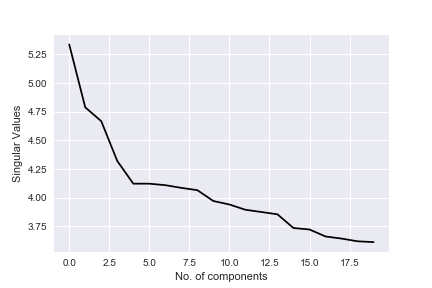
\includegraphics[width=1\linewidth]{figures/singular_values_log_yscale}
    \caption{\small Top 20 singular values (SVD). Log-scale on y-axis for better visualization.}
    \label{fig:svd}
\end{subfigure}%
\begin{subfigure}{.5\textwidth}
    \centering
    \includegraphics[width=1\linewidth]{figures/roc}
    \caption{\small ROC curve for various matrix completion methods.}
    \label{fig:roc}
\end{subfigure}
\caption{\small Scree plot and ROC curves for matrix completion methods.}
\label{fig:test}
\end{figure}

\section{Discussion}

Our analysis showed that NMF outperforms SVD and LDA on metrics described in the results section. Moreover, it was observed that LDA was extremely slow even when the number of topics was as small as 5. This could possibly be due to the underlying algorithmic implementation of LDA which is more suited for topic modelling in text documents by iterating over all the words in a document for all the documents in a corpus. The high dimensionality of our dataset makes it computationally intractable to train for larger number of topics.

Two supervised learning methods also worked well. In particular, logistic regression was extremely fast on subsamples of a full dataset of graph-based features. We found that the proportion of positive examples was an important hyperparameter. The model had better accuracy with a lower proportion of positive examples, but a slightly worse recall.

We have therefore approached the task of identifying whether a transaction will occur from two angles. The first viewpoint leverages classification techniques such as SVM and Logistic regression by constructing features from the training dataset using graph properties of indegree and outdegree. The second approach involves viewing the data as a large and sparse matrix of the counts of transactions and employing matrix completion methods like NMF, SVD and LDA to get a low rank approximation of the data and thereby identify the underlying latent structures. In conclusion, the future direction of this work can involve developing complex models which make use of both the classification and matrix completion methods in conjunction with each other so as to better predict transactions.

\subsubsection*{Acknowledgments}

We benefited from class notes, precept discussion, and office hours for Princeton's COS 424.

\bibliography{ref}
\bibliographystyle{plain}

\end{document}
